\documentclass[letterpaper,12pt]{article}
\usepackage[margin=.65in,top=.72in,bottom=.62in,headheight=16pt,headsep=15pt,footskip=19pt]{geometry}
\usepackage[T1]{fontenc}
\usepackage{lmodern,tikz,fancyhdr}\pdfmapfile{+lm.map}
\usetikzlibrary{arrows.meta,shapes.geometric}
\pagestyle{fancy}\fancyhf{}\renewcommand{\headrulewidth}{0pt}\renewcommand{\footrulewidth}{0pt}
\setlength{\parindent}{0pt}\setlength{\parskip}{0pt}
\fancyhead[L]{\small Week 43 / Shuffling picture cards / Grades 2--3}
\fancyfoot[L]{\footnotesize Bellingham Math Circle / Week 43 / W43-grades-2-3-v2}\fancyfoot[R]{\footnotesize\thepage}
\begin{document}
\noindent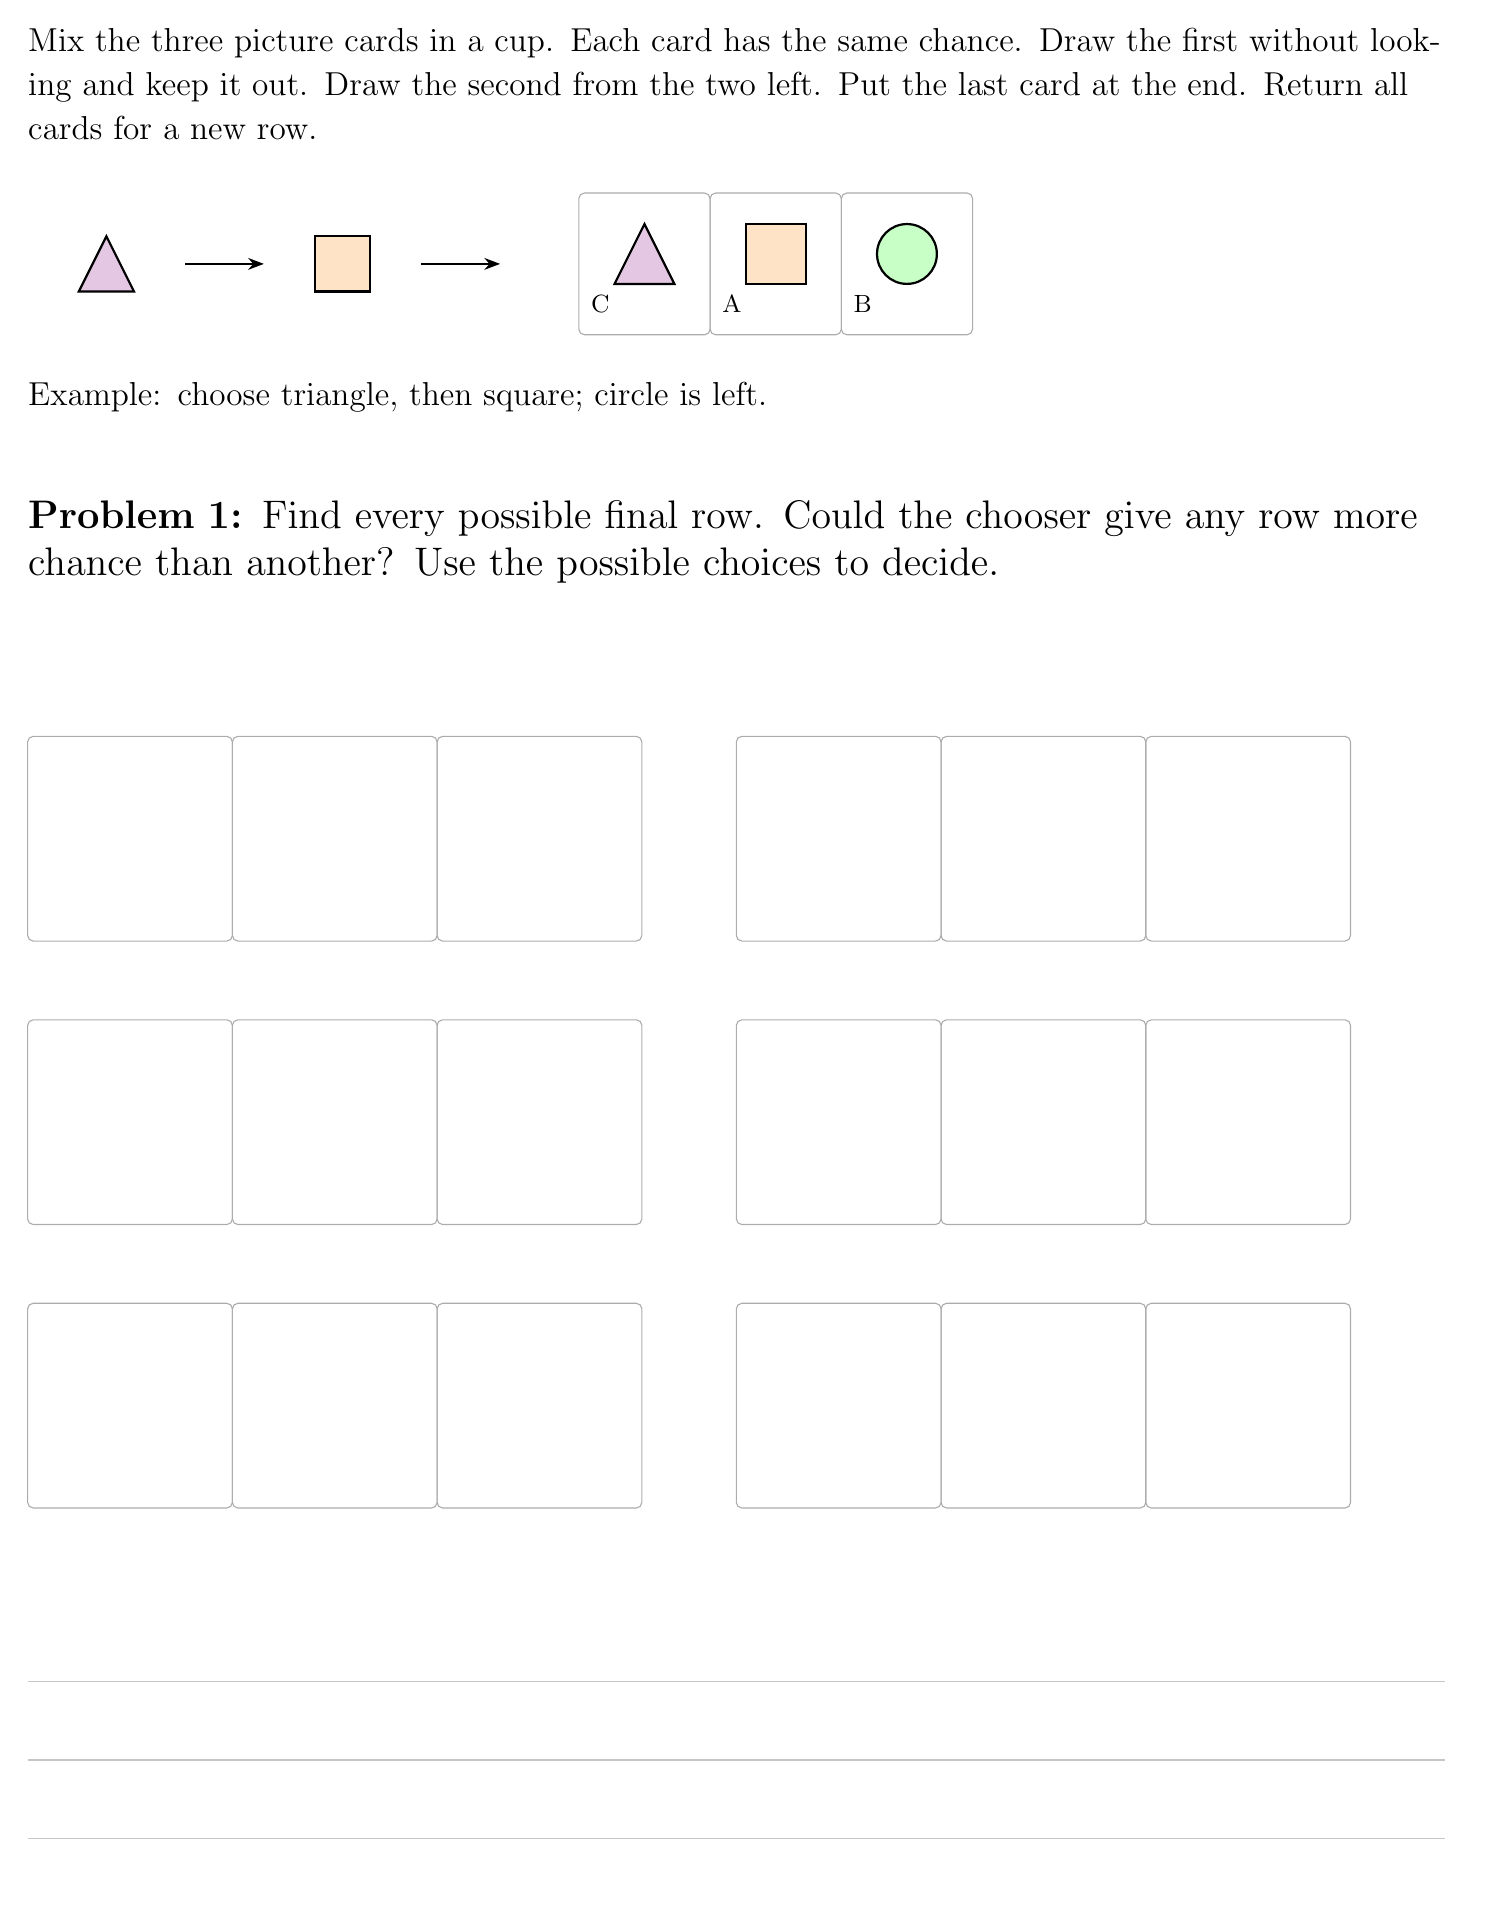
\begin{tikzpicture}[x=1cm,y=1cm]\path[use as bounding box] (0,0) rectangle (18.2,-23.6);
\node[anchor=north west,text width=18cm,inner sep=0pt,font=\fontsize{13}{16}\selectfont] at (0,0) {Mix the three picture cards in a cup. Each card has the same chance. Draw the first without looking and keep it out. Draw the second from the two left. Put the last card at the end. Return all cards for a new row.};
\draw[fill=violet!22,line width=.8pt] (1,-2.65) -- (1.35,-3.35) -- (0.65,-3.35) -- cycle;
\draw[-{Stealth[length=2mm]},line width=.8pt] (2,-3) -- (3,-3) node[midway,above,font=\small] {};
\draw[fill=orange!22,line width=.8pt] (3.65,-3.35) rectangle (4.35,-2.65);
\draw[-{Stealth[length=2mm]},line width=.8pt] (5,-3) -- (6,-3) node[midway,above,font=\small] {};
\draw[gray!65,rounded corners=2pt] (7.0,-2.1) rectangle (8.666666666666666,-3.9000000000000004);
\draw[fill=violet!22,line width=.8pt] (7.833333333333333,-2.494) -- (8.213333333333333,-3.254) -- (7.453333333333333,-3.254) -- cycle;
\node[anchor=north west,text width=1.4666666666666668cm,inner sep=0pt,font=\fontsize{9}{12}\selectfont] at (7.15,-3.396) {C};
\draw[gray!65,rounded corners=2pt] (8.666666666666666,-2.1) rectangle (10.333333333333332,-3.9000000000000004);
\draw[fill=orange!22,line width=.8pt] (9.12,-3.254) rectangle (9.88,-2.494);
\node[anchor=north west,text width=1.4666666666666668cm,inner sep=0pt,font=\fontsize{9}{12}\selectfont] at (8.816666666666666,-3.396) {A};
\draw[gray!65,rounded corners=2pt] (10.333333333333334,-2.1) rectangle (12.0,-3.9000000000000004);
\draw[fill=green!22,line width=.8pt] (11.166666666666668,-2.874) circle (0.38);
\node[anchor=north west,text width=1.4666666666666668cm,inner sep=0pt,font=\fontsize{9}{12}\selectfont] at (10.483333333333334,-3.396) {B};
\node[anchor=north west,text width=18cm,inner sep=0pt,font=\fontsize{12}{15}\selectfont] at (0,-4.5) {Example: choose triangle, then square; circle is left.};
\node[anchor=north west,text width=18cm,inner sep=0pt,font=\fontsize{14}{17}\selectfont] at (0,-6) {\textbf{Problem 1:} Find every possible final row. Could the chooser give any row more chance than another? Use the possible choices to decide.};
\draw[gray!65,rounded corners=2pt] (0.0,-9.0) rectangle (2.6,-11.6);
\draw[gray!65,rounded corners=2pt] (2.6,-9.0) rectangle (5.2,-11.6);
\draw[gray!65,rounded corners=2pt] (5.2,-9.0) rectangle (7.800000000000001,-11.6);
\draw[gray!65,rounded corners=2pt] (9.0,-9.0) rectangle (11.6,-11.6);
\draw[gray!65,rounded corners=2pt] (11.6,-9.0) rectangle (14.2,-11.6);
\draw[gray!65,rounded corners=2pt] (14.2,-9.0) rectangle (16.8,-11.6);
\draw[gray!65,rounded corners=2pt] (0.0,-12.6) rectangle (2.6,-15.2);
\draw[gray!65,rounded corners=2pt] (2.6,-12.6) rectangle (5.2,-15.2);
\draw[gray!65,rounded corners=2pt] (5.2,-12.6) rectangle (7.800000000000001,-15.2);
\draw[gray!65,rounded corners=2pt] (9.0,-12.6) rectangle (11.6,-15.2);
\draw[gray!65,rounded corners=2pt] (11.6,-12.6) rectangle (14.2,-15.2);
\draw[gray!65,rounded corners=2pt] (14.2,-12.6) rectangle (16.8,-15.2);
\draw[gray!65,rounded corners=2pt] (0.0,-16.2) rectangle (2.6,-18.8);
\draw[gray!65,rounded corners=2pt] (2.6,-16.2) rectangle (5.2,-18.8);
\draw[gray!65,rounded corners=2pt] (5.2,-16.2) rectangle (7.800000000000001,-18.8);
\draw[gray!65,rounded corners=2pt] (9.0,-16.2) rectangle (11.6,-18.8);
\draw[gray!65,rounded corners=2pt] (11.6,-16.2) rectangle (14.2,-18.8);
\draw[gray!65,rounded corners=2pt] (14.2,-16.2) rectangle (16.8,-18.8);
\draw[gray!45] (0,-21) -- (18,-21);
\draw[gray!45] (0,-22) -- (18,-22);
\draw[gray!45] (0,-23) -- (18,-23);
\end{tikzpicture}
\newpage
\noindent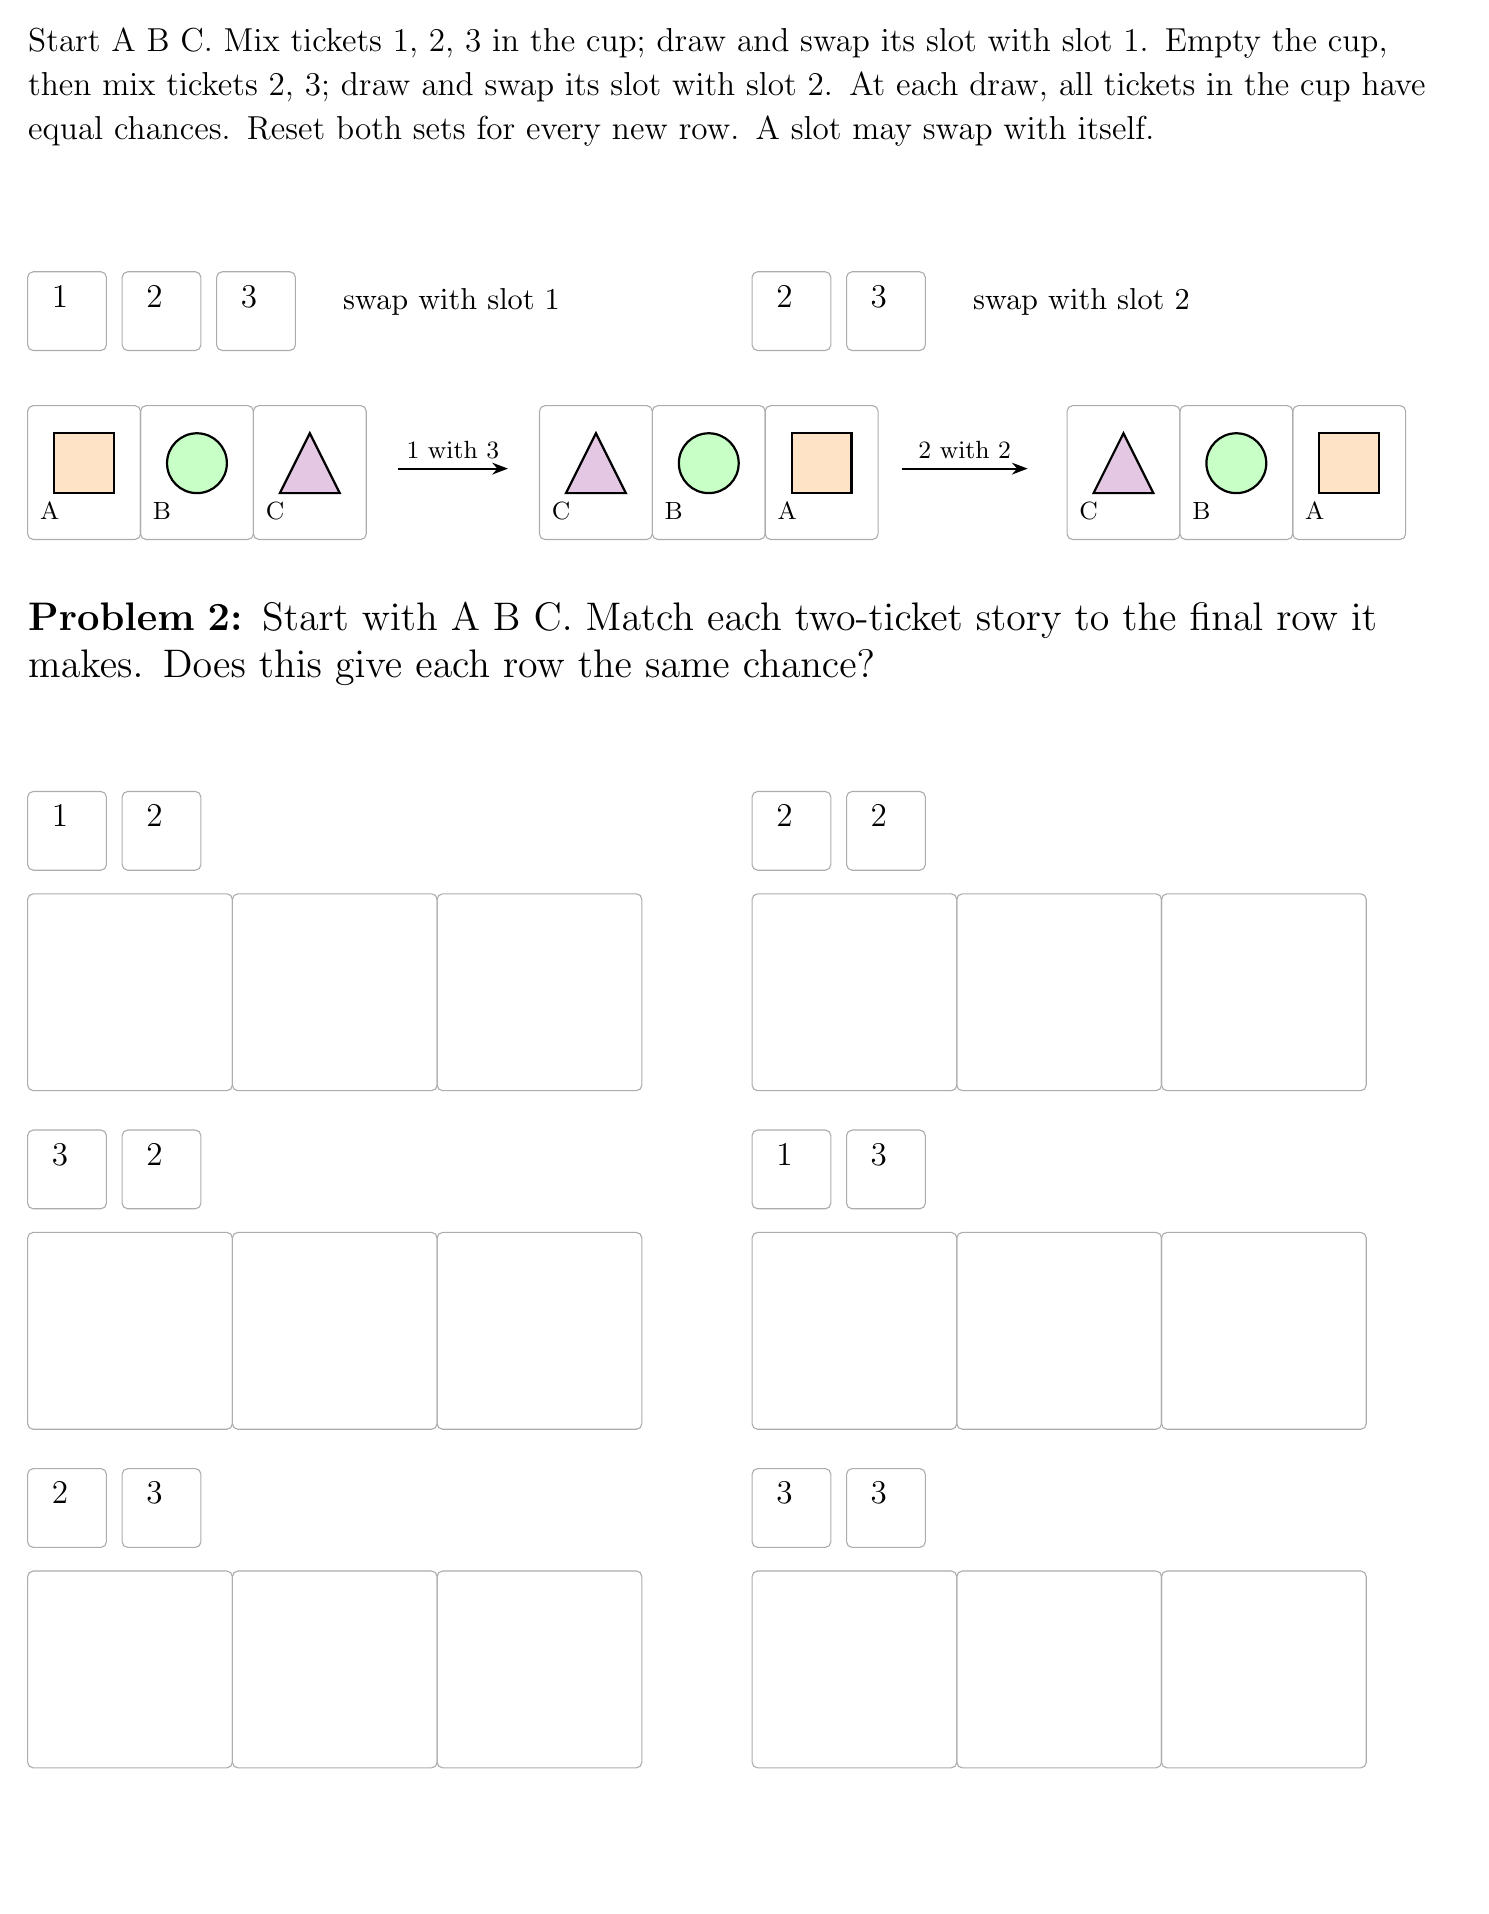
\begin{tikzpicture}[x=1cm,y=1cm]\path[use as bounding box] (0,0) rectangle (18.2,-23.6);
\node[anchor=north west,text width=18cm,inner sep=0pt,font=\fontsize{13}{16}\selectfont] at (0,0) {Start A B C. Mix tickets 1, 2, 3 in the cup; draw and swap its slot with slot 1. Empty the cup, then mix tickets 2, 3; draw and swap its slot with slot 2. At each draw, all tickets in the cup have equal chances. Reset both sets for every new row. A slot may swap with itself.};
\draw[gray!65,rounded corners=2pt] (0.0,-3.1) rectangle (1.0,-4.1);
\node[anchor=north west,text width=0.5cm,inner sep=0pt,font=\fontsize{13}{16}\selectfont] at (0.3,-3.27) {1};
\draw[gray!65,rounded corners=2pt] (1.2,-3.1) rectangle (2.2,-4.1);
\node[anchor=north west,text width=0.5cm,inner sep=0pt,font=\fontsize{13}{16}\selectfont] at (1.5,-3.27) {2};
\draw[gray!65,rounded corners=2pt] (2.4,-3.1) rectangle (3.4,-4.1);
\node[anchor=north west,text width=0.5cm,inner sep=0pt,font=\fontsize{13}{16}\selectfont] at (2.6999999999999997,-3.27) {3};
\node[anchor=north west,text width=5cm,inner sep=0pt,font=\fontsize{11}{14}\selectfont] at (4,-3.3) {swap with slot 1};
\draw[gray!65,rounded corners=2pt] (9.2,-3.1) rectangle (10.2,-4.1);
\node[anchor=north west,text width=0.5cm,inner sep=0pt,font=\fontsize{13}{16}\selectfont] at (9.5,-3.27) {2};
\draw[gray!65,rounded corners=2pt] (10.399999999999999,-3.1) rectangle (11.399999999999999,-4.1);
\node[anchor=north west,text width=0.5cm,inner sep=0pt,font=\fontsize{13}{16}\selectfont] at (10.7,-3.27) {3};
\node[anchor=north west,text width=6cm,inner sep=0pt,font=\fontsize{11}{14}\selectfont] at (12,-3.3) {swap with slot 2};
\draw[gray!65,rounded corners=2pt] (0.0,-4.8) rectangle (1.4333333333333333,-6.5);
\draw[fill=orange!22,line width=.8pt] (0.33666666666666667,-5.911) rectangle (1.0966666666666667,-5.151);
\node[anchor=north west,text width=1.2333333333333334cm,inner sep=0pt,font=\fontsize{9}{12}\selectfont] at (0.15,-6.024) {A};
\draw[gray!65,rounded corners=2pt] (1.4333333333333333,-4.8) rectangle (2.8666666666666667,-6.5);
\draw[fill=green!22,line width=.8pt] (2.15,-5.531) circle (0.38);
\node[anchor=north west,text width=1.2333333333333334cm,inner sep=0pt,font=\fontsize{9}{12}\selectfont] at (1.5833333333333333,-6.024) {B};
\draw[gray!65,rounded corners=2pt] (2.8666666666666667,-4.8) rectangle (4.3,-6.5);
\draw[fill=violet!22,line width=.8pt] (3.5833333333333335,-5.151) -- (3.9633333333333334,-5.911) -- (3.2033333333333336,-5.911) -- cycle;
\node[anchor=north west,text width=1.2333333333333334cm,inner sep=0pt,font=\fontsize{9}{12}\selectfont] at (3.0166666666666666,-6.024) {C};
\draw[-{Stealth[length=2mm]},line width=.8pt] (4.7,-5.6) -- (6.1,-5.6) node[midway,above,font=\small] {1 with 3};
\draw[gray!65,rounded corners=2pt] (6.5,-4.8) rectangle (7.933333333333334,-6.5);
\draw[fill=violet!22,line width=.8pt] (7.216666666666667,-5.151) -- (7.596666666666667,-5.911) -- (6.836666666666667,-5.911) -- cycle;
\node[anchor=north west,text width=1.2333333333333334cm,inner sep=0pt,font=\fontsize{9}{12}\selectfont] at (6.65,-6.024) {C};
\draw[gray!65,rounded corners=2pt] (7.933333333333334,-4.8) rectangle (9.366666666666667,-6.5);
\draw[fill=green!22,line width=.8pt] (8.65,-5.531) circle (0.38);
\node[anchor=north west,text width=1.2333333333333334cm,inner sep=0pt,font=\fontsize{9}{12}\selectfont] at (8.083333333333334,-6.024) {B};
\draw[gray!65,rounded corners=2pt] (9.366666666666667,-4.8) rectangle (10.8,-6.5);
\draw[fill=orange!22,line width=.8pt] (9.703333333333333,-5.911) rectangle (10.463333333333335,-5.151);
\node[anchor=north west,text width=1.2333333333333334cm,inner sep=0pt,font=\fontsize{9}{12}\selectfont] at (9.516666666666667,-6.024) {A};
\draw[-{Stealth[length=2mm]},line width=.8pt] (11.1,-5.6) -- (12.7,-5.6) node[midway,above,font=\small] {2 with 2};
\draw[gray!65,rounded corners=2pt] (13.2,-4.8) rectangle (14.633333333333333,-6.5);
\draw[fill=violet!22,line width=.8pt] (13.916666666666666,-5.151) -- (14.296666666666667,-5.911) -- (13.536666666666665,-5.911) -- cycle;
\node[anchor=north west,text width=1.2333333333333334cm,inner sep=0pt,font=\fontsize{9}{12}\selectfont] at (13.35,-6.024) {C};
\draw[gray!65,rounded corners=2pt] (14.633333333333333,-4.8) rectangle (16.066666666666666,-6.5);
\draw[fill=green!22,line width=.8pt] (15.35,-5.531) circle (0.38);
\node[anchor=north west,text width=1.2333333333333334cm,inner sep=0pt,font=\fontsize{9}{12}\selectfont] at (14.783333333333333,-6.024) {B};
\draw[gray!65,rounded corners=2pt] (16.066666666666666,-4.8) rectangle (17.5,-6.5);
\draw[fill=orange!22,line width=.8pt] (16.403333333333332,-5.911) rectangle (17.16333333333333,-5.151);
\node[anchor=north west,text width=1.2333333333333334cm,inner sep=0pt,font=\fontsize{9}{12}\selectfont] at (16.216666666666665,-6.024) {A};
\node[anchor=north west,text width=18cm,inner sep=0pt,font=\fontsize{14}{17}\selectfont] at (0,-7.3) {\textbf{Problem 2:} Start with A B C. Match each two-ticket story to the final row it makes. Does this give each row the same chance?};
\draw[gray!65,rounded corners=2pt] (0.0,-9.7) rectangle (1.0,-10.7);
\node[anchor=north west,text width=0.5cm,inner sep=0pt,font=\fontsize{13}{16}\selectfont] at (0.3,-9.87) {1};
\draw[gray!65,rounded corners=2pt] (1.2,-9.7) rectangle (2.2,-10.7);
\node[anchor=north west,text width=0.5cm,inner sep=0pt,font=\fontsize{13}{16}\selectfont] at (1.5,-9.87) {2};
\draw[gray!65,rounded corners=2pt] (0.0,-11.0) rectangle (2.6,-13.5);
\draw[gray!65,rounded corners=2pt] (2.6,-11.0) rectangle (5.2,-13.5);
\draw[gray!65,rounded corners=2pt] (5.2,-11.0) rectangle (7.800000000000001,-13.5);
\draw[gray!65,rounded corners=2pt] (9.2,-9.7) rectangle (10.2,-10.7);
\node[anchor=north west,text width=0.5cm,inner sep=0pt,font=\fontsize{13}{16}\selectfont] at (9.5,-9.87) {2};
\draw[gray!65,rounded corners=2pt] (10.399999999999999,-9.7) rectangle (11.399999999999999,-10.7);
\node[anchor=north west,text width=0.5cm,inner sep=0pt,font=\fontsize{13}{16}\selectfont] at (10.7,-9.87) {2};
\draw[gray!65,rounded corners=2pt] (9.2,-11.0) rectangle (11.799999999999999,-13.5);
\draw[gray!65,rounded corners=2pt] (11.799999999999999,-11.0) rectangle (14.399999999999999,-13.5);
\draw[gray!65,rounded corners=2pt] (14.399999999999999,-11.0) rectangle (17.0,-13.5);
\draw[gray!65,rounded corners=2pt] (0.0,-14.0) rectangle (1.0,-15.0);
\node[anchor=north west,text width=0.5cm,inner sep=0pt,font=\fontsize{13}{16}\selectfont] at (0.3,-14.17) {3};
\draw[gray!65,rounded corners=2pt] (1.2,-14.0) rectangle (2.2,-15.0);
\node[anchor=north west,text width=0.5cm,inner sep=0pt,font=\fontsize{13}{16}\selectfont] at (1.5,-14.17) {2};
\draw[gray!65,rounded corners=2pt] (0.0,-15.3) rectangle (2.6,-17.8);
\draw[gray!65,rounded corners=2pt] (2.6,-15.3) rectangle (5.2,-17.8);
\draw[gray!65,rounded corners=2pt] (5.2,-15.3) rectangle (7.800000000000001,-17.8);
\draw[gray!65,rounded corners=2pt] (9.2,-14.0) rectangle (10.2,-15.0);
\node[anchor=north west,text width=0.5cm,inner sep=0pt,font=\fontsize{13}{16}\selectfont] at (9.5,-14.17) {1};
\draw[gray!65,rounded corners=2pt] (10.399999999999999,-14.0) rectangle (11.399999999999999,-15.0);
\node[anchor=north west,text width=0.5cm,inner sep=0pt,font=\fontsize{13}{16}\selectfont] at (10.7,-14.17) {3};
\draw[gray!65,rounded corners=2pt] (9.2,-15.3) rectangle (11.799999999999999,-17.8);
\draw[gray!65,rounded corners=2pt] (11.799999999999999,-15.3) rectangle (14.399999999999999,-17.8);
\draw[gray!65,rounded corners=2pt] (14.399999999999999,-15.3) rectangle (17.0,-17.8);
\draw[gray!65,rounded corners=2pt] (0.0,-18.299999999999997) rectangle (1.0,-19.299999999999997);
\node[anchor=north west,text width=0.5cm,inner sep=0pt,font=\fontsize{13}{16}\selectfont] at (0.3,-18.47) {2};
\draw[gray!65,rounded corners=2pt] (1.2,-18.299999999999997) rectangle (2.2,-19.299999999999997);
\node[anchor=north west,text width=0.5cm,inner sep=0pt,font=\fontsize{13}{16}\selectfont] at (1.5,-18.47) {3};
\draw[gray!65,rounded corners=2pt] (0.0,-19.599999999999998) rectangle (2.6,-22.099999999999998);
\draw[gray!65,rounded corners=2pt] (2.6,-19.599999999999998) rectangle (5.2,-22.099999999999998);
\draw[gray!65,rounded corners=2pt] (5.2,-19.599999999999998) rectangle (7.800000000000001,-22.099999999999998);
\draw[gray!65,rounded corners=2pt] (9.2,-18.299999999999997) rectangle (10.2,-19.299999999999997);
\node[anchor=north west,text width=0.5cm,inner sep=0pt,font=\fontsize{13}{16}\selectfont] at (9.5,-18.47) {3};
\draw[gray!65,rounded corners=2pt] (10.399999999999999,-18.299999999999997) rectangle (11.399999999999999,-19.299999999999997);
\node[anchor=north west,text width=0.5cm,inner sep=0pt,font=\fontsize{13}{16}\selectfont] at (10.7,-18.47) {3};
\draw[gray!65,rounded corners=2pt] (9.2,-19.599999999999998) rectangle (11.799999999999999,-22.099999999999998);
\draw[gray!65,rounded corners=2pt] (11.799999999999999,-19.599999999999998) rectangle (14.399999999999999,-22.099999999999998);
\draw[gray!65,rounded corners=2pt] (14.399999999999999,-19.599999999999998) rectangle (17.0,-22.099999999999998);
\end{tikzpicture}
\newpage
\noindent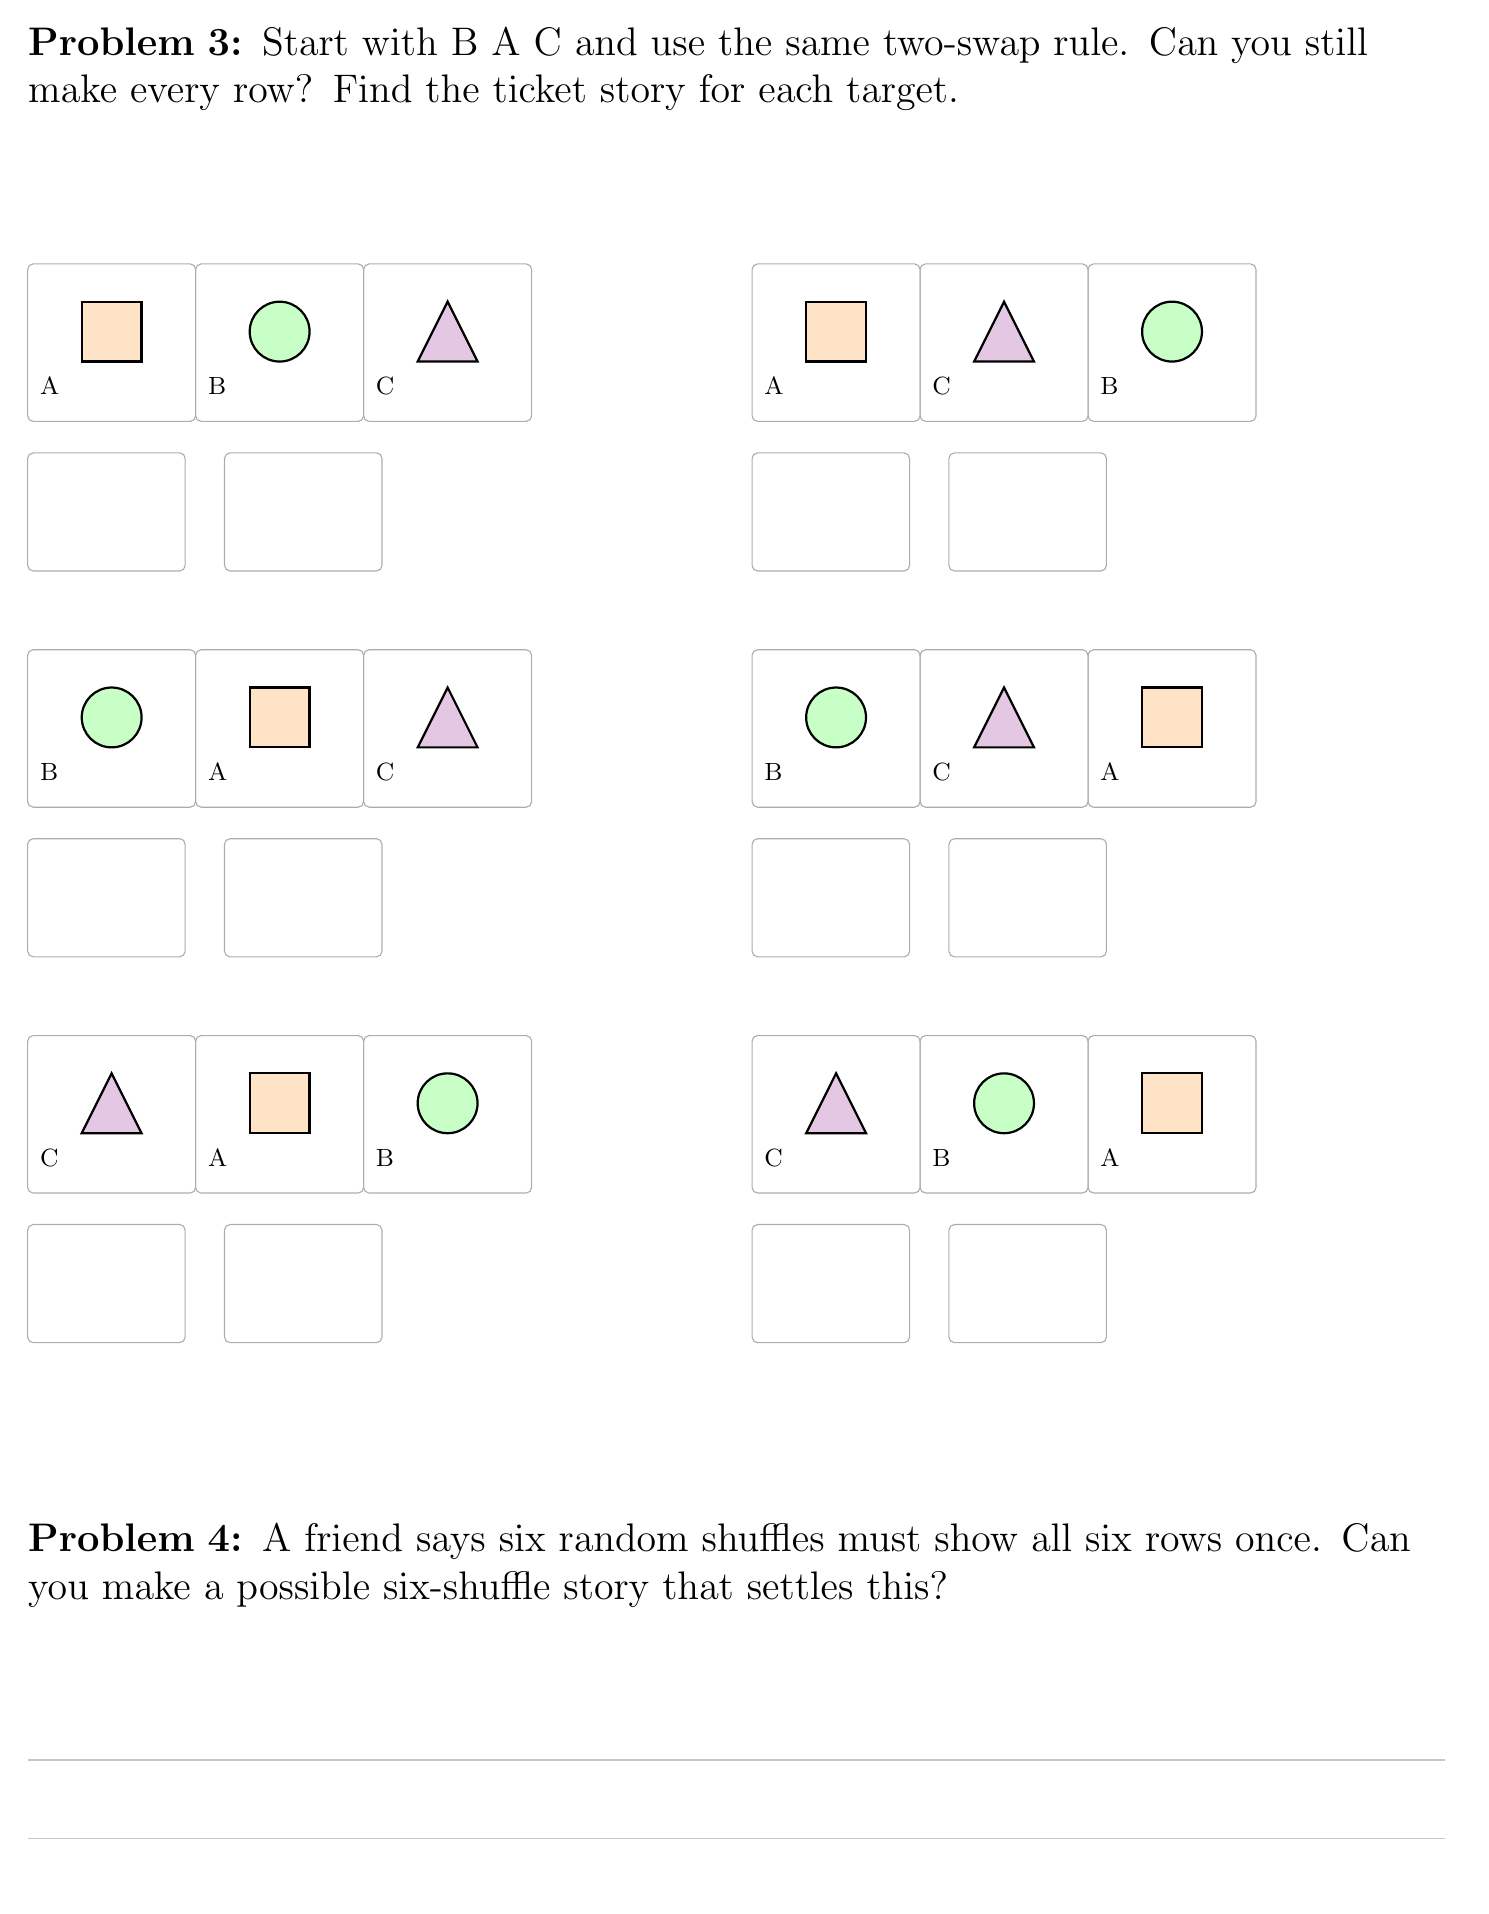
\begin{tikzpicture}[x=1cm,y=1cm]\path[use as bounding box] (0,0) rectangle (18.2,-23.6);
\node[anchor=north west,text width=18cm,inner sep=0pt,font=\fontsize{14}{17}\selectfont] at (0,0) {\textbf{Problem 3:} Start with B A C and use the same two-swap rule. Can you still make every row? Find the ticket story for each target.};
\draw[gray!65,rounded corners=2pt] (0.0,-3.0) rectangle (2.1333333333333333,-5.0);
\draw[fill=orange!22,line width=.8pt] (0.6866666666666666,-4.24) rectangle (1.4466666666666668,-3.48);
\node[anchor=north west,text width=1.9333333333333333cm,inner sep=0pt,font=\fontsize{9}{12}\selectfont] at (0.15,-4.4399999999999995) {A};
\draw[gray!65,rounded corners=2pt] (2.1333333333333333,-3.0) rectangle (4.266666666666667,-5.0);
\draw[fill=green!22,line width=.8pt] (3.2000000000000006,-3.86) circle (0.38);
\node[anchor=north west,text width=1.9333333333333333cm,inner sep=0pt,font=\fontsize{9}{12}\selectfont] at (2.283333333333333,-4.4399999999999995) {B};
\draw[gray!65,rounded corners=2pt] (4.266666666666667,-3.0) rectangle (6.4,-5.0);
\draw[fill=violet!22,line width=.8pt] (5.333333333333333,-3.48) -- (5.713333333333333,-4.24) -- (4.953333333333333,-4.24) -- cycle;
\node[anchor=north west,text width=1.9333333333333333cm,inner sep=0pt,font=\fontsize{9}{12}\selectfont] at (4.416666666666667,-4.4399999999999995) {C};
\draw[gray!65,rounded corners=2pt] (0.0,-5.4) rectangle (2.0,-6.9);
\draw[gray!65,rounded corners=2pt] (2.5,-5.4) rectangle (4.5,-6.9);
\draw[gray!65,rounded corners=2pt] (9.2,-3.0) rectangle (11.333333333333332,-5.0);
\draw[fill=orange!22,line width=.8pt] (9.886666666666665,-4.24) rectangle (10.646666666666667,-3.48);
\node[anchor=north west,text width=1.9333333333333333cm,inner sep=0pt,font=\fontsize{9}{12}\selectfont] at (9.35,-4.4399999999999995) {A};
\draw[gray!65,rounded corners=2pt] (11.333333333333332,-3.0) rectangle (13.466666666666665,-5.0);
\draw[fill=violet!22,line width=.8pt] (12.4,-3.48) -- (12.780000000000001,-4.24) -- (12.02,-4.24) -- cycle;
\node[anchor=north west,text width=1.9333333333333333cm,inner sep=0pt,font=\fontsize{9}{12}\selectfont] at (11.483333333333333,-4.4399999999999995) {C};
\draw[gray!65,rounded corners=2pt] (13.466666666666665,-3.0) rectangle (15.599999999999998,-5.0);
\draw[fill=green!22,line width=.8pt] (14.533333333333331,-3.86) circle (0.38);
\node[anchor=north west,text width=1.9333333333333333cm,inner sep=0pt,font=\fontsize{9}{12}\selectfont] at (13.616666666666665,-4.4399999999999995) {B};
\draw[gray!65,rounded corners=2pt] (9.2,-5.4) rectangle (11.2,-6.9);
\draw[gray!65,rounded corners=2pt] (11.7,-5.4) rectangle (13.7,-6.9);
\draw[gray!65,rounded corners=2pt] (0.0,-7.9) rectangle (2.1333333333333333,-9.9);
\draw[fill=green!22,line width=.8pt] (1.0666666666666667,-8.76) circle (0.38);
\node[anchor=north west,text width=1.9333333333333333cm,inner sep=0pt,font=\fontsize{9}{12}\selectfont] at (0.15,-9.34) {B};
\draw[gray!65,rounded corners=2pt] (2.1333333333333333,-7.9) rectangle (4.266666666666667,-9.9);
\draw[fill=orange!22,line width=.8pt] (2.8200000000000007,-9.14) rectangle (3.5800000000000005,-8.379999999999999);
\node[anchor=north west,text width=1.9333333333333333cm,inner sep=0pt,font=\fontsize{9}{12}\selectfont] at (2.283333333333333,-9.34) {A};
\draw[gray!65,rounded corners=2pt] (4.266666666666667,-7.9) rectangle (6.4,-9.9);
\draw[fill=violet!22,line width=.8pt] (5.333333333333333,-8.379999999999999) -- (5.713333333333333,-9.14) -- (4.953333333333333,-9.14) -- cycle;
\node[anchor=north west,text width=1.9333333333333333cm,inner sep=0pt,font=\fontsize{9}{12}\selectfont] at (4.416666666666667,-9.34) {C};
\draw[gray!65,rounded corners=2pt] (0.0,-10.3) rectangle (2.0,-11.8);
\draw[gray!65,rounded corners=2pt] (2.5,-10.3) rectangle (4.5,-11.8);
\draw[gray!65,rounded corners=2pt] (9.2,-7.9) rectangle (11.333333333333332,-9.9);
\draw[fill=green!22,line width=.8pt] (10.266666666666666,-8.76) circle (0.38);
\node[anchor=north west,text width=1.9333333333333333cm,inner sep=0pt,font=\fontsize{9}{12}\selectfont] at (9.35,-9.34) {B};
\draw[gray!65,rounded corners=2pt] (11.333333333333332,-7.9) rectangle (13.466666666666665,-9.9);
\draw[fill=violet!22,line width=.8pt] (12.4,-8.379999999999999) -- (12.780000000000001,-9.14) -- (12.02,-9.14) -- cycle;
\node[anchor=north west,text width=1.9333333333333333cm,inner sep=0pt,font=\fontsize{9}{12}\selectfont] at (11.483333333333333,-9.34) {C};
\draw[gray!65,rounded corners=2pt] (13.466666666666665,-7.9) rectangle (15.599999999999998,-9.9);
\draw[fill=orange!22,line width=.8pt] (14.15333333333333,-9.14) rectangle (14.913333333333332,-8.379999999999999);
\node[anchor=north west,text width=1.9333333333333333cm,inner sep=0pt,font=\fontsize{9}{12}\selectfont] at (13.616666666666665,-9.34) {A};
\draw[gray!65,rounded corners=2pt] (9.2,-10.3) rectangle (11.2,-11.8);
\draw[gray!65,rounded corners=2pt] (11.7,-10.3) rectangle (13.7,-11.8);
\draw[gray!65,rounded corners=2pt] (0.0,-12.8) rectangle (2.1333333333333333,-14.8);
\draw[fill=violet!22,line width=.8pt] (1.0666666666666667,-13.28) -- (1.4466666666666668,-14.040000000000001) -- (0.6866666666666666,-14.040000000000001) -- cycle;
\node[anchor=north west,text width=1.9333333333333333cm,inner sep=0pt,font=\fontsize{9}{12}\selectfont] at (0.15,-14.24) {C};
\draw[gray!65,rounded corners=2pt] (2.1333333333333333,-12.8) rectangle (4.266666666666667,-14.8);
\draw[fill=orange!22,line width=.8pt] (2.8200000000000007,-14.040000000000001) rectangle (3.5800000000000005,-13.28);
\node[anchor=north west,text width=1.9333333333333333cm,inner sep=0pt,font=\fontsize{9}{12}\selectfont] at (2.283333333333333,-14.24) {A};
\draw[gray!65,rounded corners=2pt] (4.266666666666667,-12.8) rectangle (6.4,-14.8);
\draw[fill=green!22,line width=.8pt] (5.333333333333333,-13.66) circle (0.38);
\node[anchor=north west,text width=1.9333333333333333cm,inner sep=0pt,font=\fontsize{9}{12}\selectfont] at (4.416666666666667,-14.24) {B};
\draw[gray!65,rounded corners=2pt] (0.0,-15.200000000000001) rectangle (2.0,-16.700000000000003);
\draw[gray!65,rounded corners=2pt] (2.5,-15.200000000000001) rectangle (4.5,-16.700000000000003);
\draw[gray!65,rounded corners=2pt] (9.2,-12.8) rectangle (11.333333333333332,-14.8);
\draw[fill=violet!22,line width=.8pt] (10.266666666666666,-13.28) -- (10.646666666666667,-14.040000000000001) -- (9.886666666666665,-14.040000000000001) -- cycle;
\node[anchor=north west,text width=1.9333333333333333cm,inner sep=0pt,font=\fontsize{9}{12}\selectfont] at (9.35,-14.24) {C};
\draw[gray!65,rounded corners=2pt] (11.333333333333332,-12.8) rectangle (13.466666666666665,-14.8);
\draw[fill=green!22,line width=.8pt] (12.4,-13.66) circle (0.38);
\node[anchor=north west,text width=1.9333333333333333cm,inner sep=0pt,font=\fontsize{9}{12}\selectfont] at (11.483333333333333,-14.24) {B};
\draw[gray!65,rounded corners=2pt] (13.466666666666665,-12.8) rectangle (15.599999999999998,-14.8);
\draw[fill=orange!22,line width=.8pt] (14.15333333333333,-14.040000000000001) rectangle (14.913333333333332,-13.28);
\node[anchor=north west,text width=1.9333333333333333cm,inner sep=0pt,font=\fontsize{9}{12}\selectfont] at (13.616666666666665,-14.24) {A};
\draw[gray!65,rounded corners=2pt] (9.2,-15.200000000000001) rectangle (11.2,-16.700000000000003);
\draw[gray!65,rounded corners=2pt] (11.7,-15.200000000000001) rectangle (13.7,-16.700000000000003);
\node[anchor=north west,text width=18cm,inner sep=0pt,font=\fontsize{14}{17}\selectfont] at (0,-19) {\textbf{Problem 4:} A friend says six random shuffles must show all six rows once. Can you make a possible six-shuffle story that settles this?};
\draw[gray!45] (0,-22) -- (18,-22);
\draw[gray!45] (0,-23) -- (18,-23);
\end{tikzpicture}
\newpage
\noindent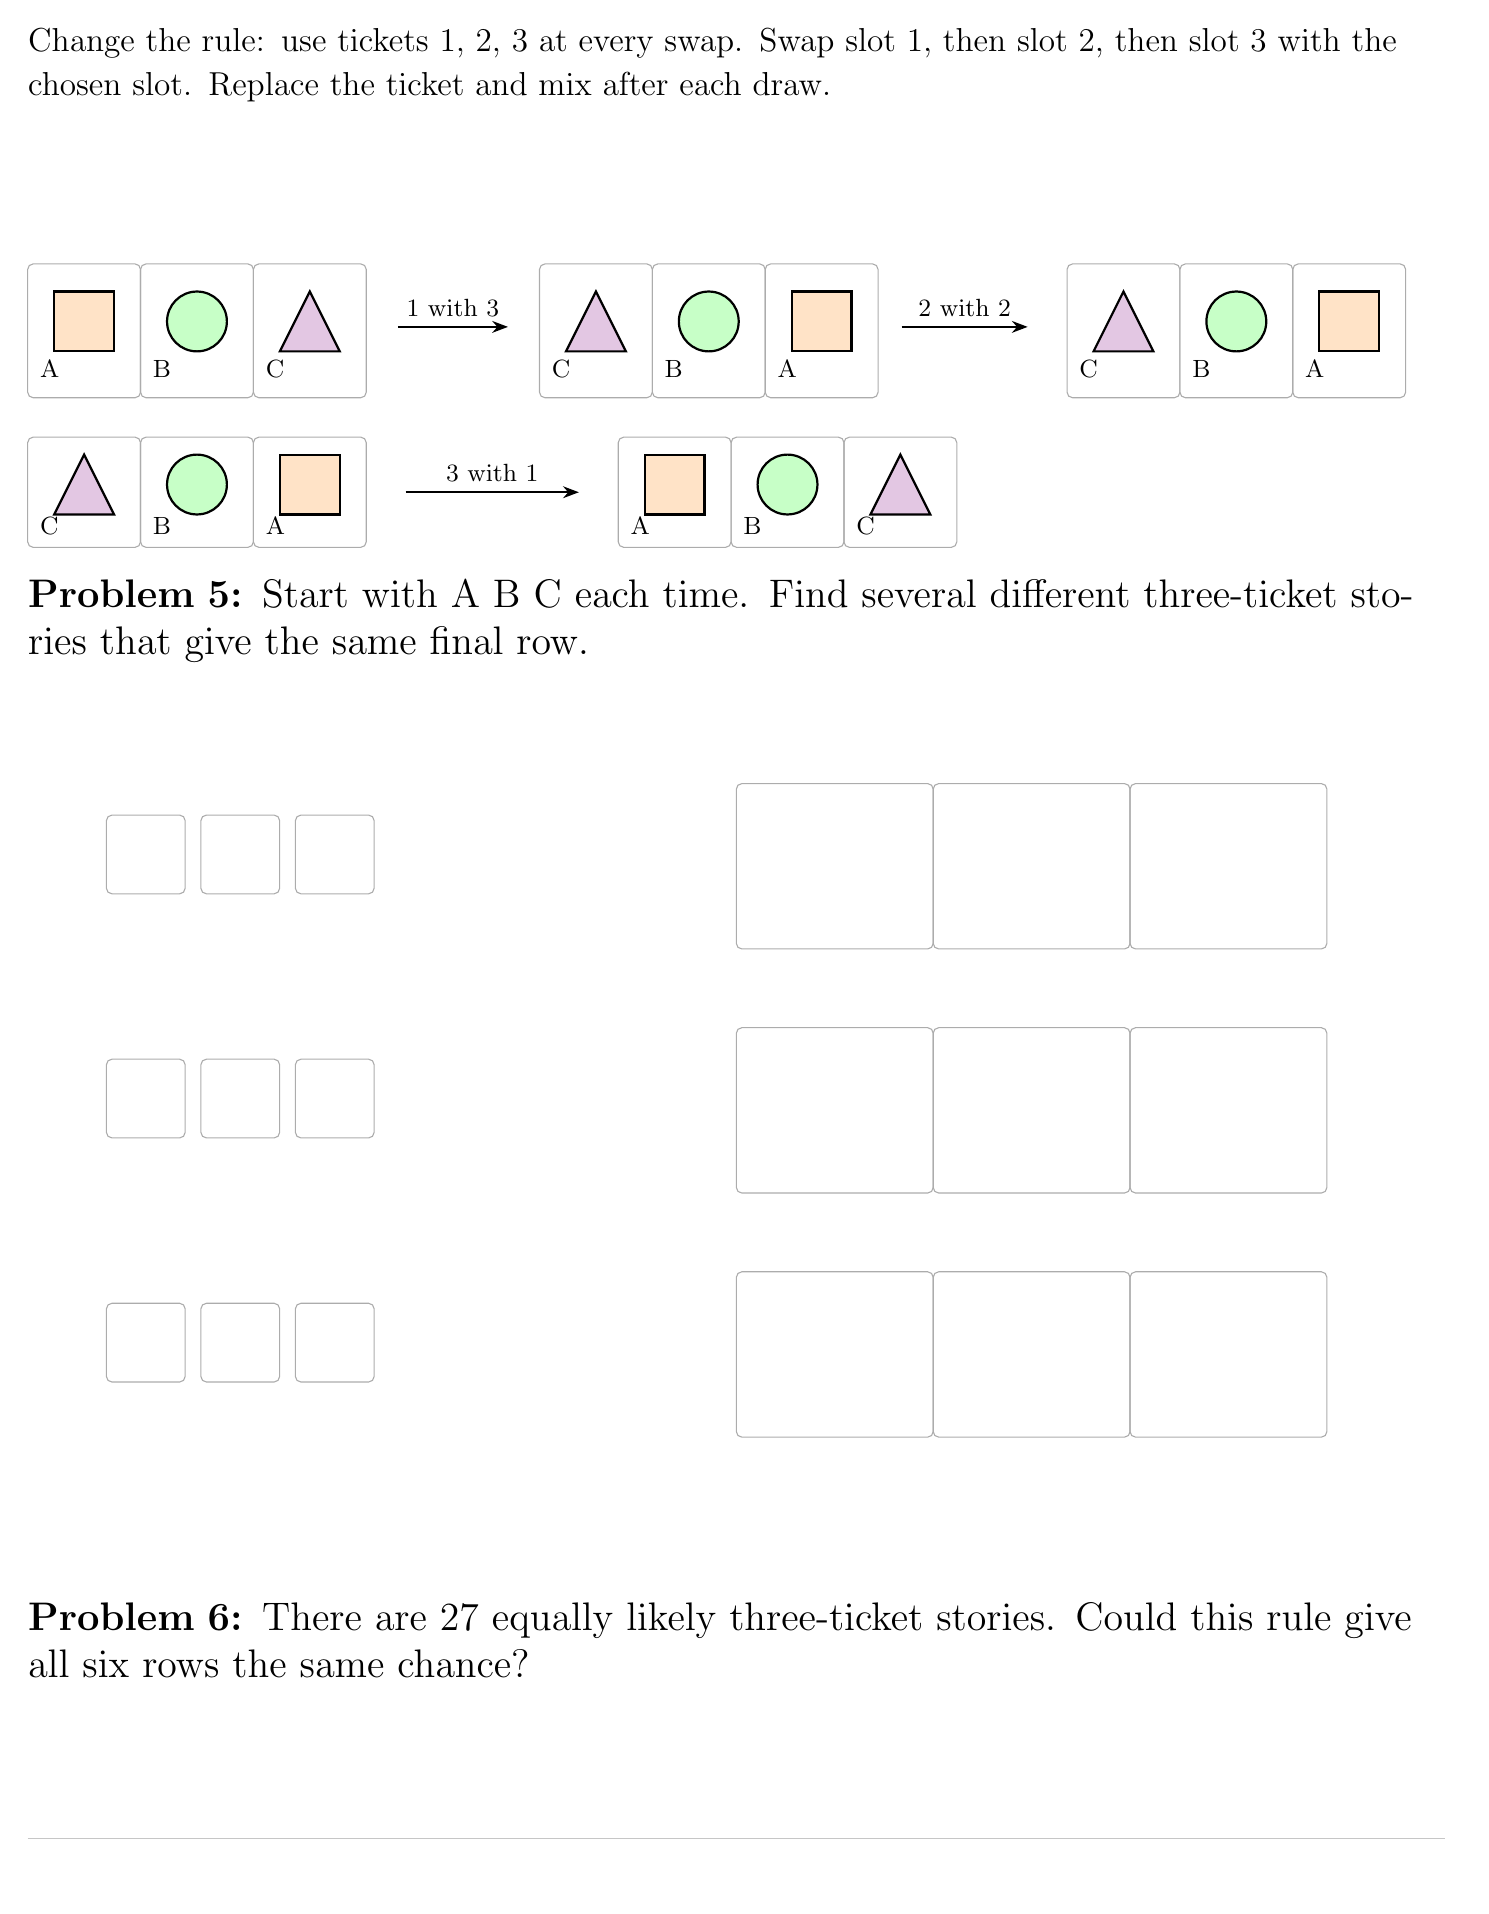
\begin{tikzpicture}[x=1cm,y=1cm]\path[use as bounding box] (0,0) rectangle (18.2,-23.6);
\node[anchor=north west,text width=18cm,inner sep=0pt,font=\fontsize{13}{16}\selectfont] at (0,0) {Change the rule: use tickets 1, 2, 3 at every swap. Swap slot 1, then slot 2, then slot 3 with the chosen slot. Replace the ticket and mix after each draw.};
\draw[gray!65,rounded corners=2pt] (0.0,-3) rectangle (1.4333333333333333,-4.7);
\draw[fill=orange!22,line width=.8pt] (0.33666666666666667,-4.111) rectangle (1.0966666666666667,-3.351);
\node[anchor=north west,text width=1.2333333333333334cm,inner sep=0pt,font=\fontsize{9}{12}\selectfont] at (0.15,-4.224) {A};
\draw[gray!65,rounded corners=2pt] (1.4333333333333333,-3) rectangle (2.8666666666666667,-4.7);
\draw[fill=green!22,line width=.8pt] (2.15,-3.731) circle (0.38);
\node[anchor=north west,text width=1.2333333333333334cm,inner sep=0pt,font=\fontsize{9}{12}\selectfont] at (1.5833333333333333,-4.224) {B};
\draw[gray!65,rounded corners=2pt] (2.8666666666666667,-3) rectangle (4.3,-4.7);
\draw[fill=violet!22,line width=.8pt] (3.5833333333333335,-3.351) -- (3.9633333333333334,-4.111) -- (3.2033333333333336,-4.111) -- cycle;
\node[anchor=north west,text width=1.2333333333333334cm,inner sep=0pt,font=\fontsize{9}{12}\selectfont] at (3.0166666666666666,-4.224) {C};
\draw[-{Stealth[length=2mm]},line width=.8pt] (4.7,-3.8) -- (6.1,-3.8) node[midway,above,font=\small] {1 with 3};
\draw[gray!65,rounded corners=2pt] (6.5,-3) rectangle (7.933333333333334,-4.7);
\draw[fill=violet!22,line width=.8pt] (7.216666666666667,-3.351) -- (7.596666666666667,-4.111) -- (6.836666666666667,-4.111) -- cycle;
\node[anchor=north west,text width=1.2333333333333334cm,inner sep=0pt,font=\fontsize{9}{12}\selectfont] at (6.65,-4.224) {C};
\draw[gray!65,rounded corners=2pt] (7.933333333333334,-3) rectangle (9.366666666666667,-4.7);
\draw[fill=green!22,line width=.8pt] (8.65,-3.731) circle (0.38);
\node[anchor=north west,text width=1.2333333333333334cm,inner sep=0pt,font=\fontsize{9}{12}\selectfont] at (8.083333333333334,-4.224) {B};
\draw[gray!65,rounded corners=2pt] (9.366666666666667,-3) rectangle (10.8,-4.7);
\draw[fill=orange!22,line width=.8pt] (9.703333333333333,-4.111) rectangle (10.463333333333335,-3.351);
\node[anchor=north west,text width=1.2333333333333334cm,inner sep=0pt,font=\fontsize{9}{12}\selectfont] at (9.516666666666667,-4.224) {A};
\draw[-{Stealth[length=2mm]},line width=.8pt] (11.1,-3.8) -- (12.7,-3.8) node[midway,above,font=\small] {2 with 2};
\draw[gray!65,rounded corners=2pt] (13.2,-3) rectangle (14.633333333333333,-4.7);
\draw[fill=violet!22,line width=.8pt] (13.916666666666666,-3.351) -- (14.296666666666667,-4.111) -- (13.536666666666665,-4.111) -- cycle;
\node[anchor=north west,text width=1.2333333333333334cm,inner sep=0pt,font=\fontsize{9}{12}\selectfont] at (13.35,-4.224) {C};
\draw[gray!65,rounded corners=2pt] (14.633333333333333,-3) rectangle (16.066666666666666,-4.7);
\draw[fill=green!22,line width=.8pt] (15.35,-3.731) circle (0.38);
\node[anchor=north west,text width=1.2333333333333334cm,inner sep=0pt,font=\fontsize{9}{12}\selectfont] at (14.783333333333333,-4.224) {B};
\draw[gray!65,rounded corners=2pt] (16.066666666666666,-3) rectangle (17.5,-4.7);
\draw[fill=orange!22,line width=.8pt] (16.403333333333332,-4.111) rectangle (17.16333333333333,-3.351);
\node[anchor=north west,text width=1.2333333333333334cm,inner sep=0pt,font=\fontsize{9}{12}\selectfont] at (16.216666666666665,-4.224) {A};
\draw[gray!65,rounded corners=2pt] (0.0,-5.2) rectangle (1.4333333333333333,-6.6);
\draw[fill=violet!22,line width=.8pt] (0.7166666666666667,-5.422000000000001) -- (1.0966666666666667,-6.182) -- (0.33666666666666667,-6.182) -- cycle;
\node[anchor=north west,text width=1.2333333333333334cm,inner sep=0pt,font=\fontsize{9}{12}\selectfont] at (0.15,-6.208) {C};
\draw[gray!65,rounded corners=2pt] (1.4333333333333333,-5.2) rectangle (2.8666666666666667,-6.6);
\draw[fill=green!22,line width=.8pt] (2.15,-5.8020000000000005) circle (0.38);
\node[anchor=north west,text width=1.2333333333333334cm,inner sep=0pt,font=\fontsize{9}{12}\selectfont] at (1.5833333333333333,-6.208) {B};
\draw[gray!65,rounded corners=2pt] (2.8666666666666667,-5.2) rectangle (4.3,-6.6);
\draw[fill=orange!22,line width=.8pt] (3.2033333333333336,-6.182) rectangle (3.9633333333333334,-5.422000000000001);
\node[anchor=north west,text width=1.2333333333333334cm,inner sep=0pt,font=\fontsize{9}{12}\selectfont] at (3.0166666666666666,-6.208) {A};
\draw[-{Stealth[length=2mm]},line width=.8pt] (4.8,-5.9) -- (7,-5.9) node[midway,above,font=\small] {3 with 1};
\draw[gray!65,rounded corners=2pt] (7.5,-5.2) rectangle (8.933333333333334,-6.6);
\draw[fill=orange!22,line width=.8pt] (7.836666666666667,-6.182) rectangle (8.596666666666668,-5.422000000000001);
\node[anchor=north west,text width=1.2333333333333334cm,inner sep=0pt,font=\fontsize{9}{12}\selectfont] at (7.65,-6.208) {A};
\draw[gray!65,rounded corners=2pt] (8.933333333333334,-5.2) rectangle (10.366666666666667,-6.6);
\draw[fill=green!22,line width=.8pt] (9.65,-5.8020000000000005) circle (0.38);
\node[anchor=north west,text width=1.2333333333333334cm,inner sep=0pt,font=\fontsize{9}{12}\selectfont] at (9.083333333333334,-6.208) {B};
\draw[gray!65,rounded corners=2pt] (10.366666666666667,-5.2) rectangle (11.8,-6.6);
\draw[fill=violet!22,line width=.8pt] (11.083333333333334,-5.422000000000001) -- (11.463333333333335,-6.182) -- (10.703333333333333,-6.182) -- cycle;
\node[anchor=north west,text width=1.2333333333333334cm,inner sep=0pt,font=\fontsize{9}{12}\selectfont] at (10.516666666666667,-6.208) {C};
\node[anchor=north west,text width=18cm,inner sep=0pt,font=\fontsize{14}{17}\selectfont] at (0,-7) {\textbf{Problem 5:} Start with A B C each time. Find several different three-ticket stories that give the same final row.};
\draw[gray!65,rounded corners=2pt] (1.0,-10.0) rectangle (2.0,-11.0);
\node[anchor=north west,text width=0.5cm,inner sep=0pt,font=\fontsize{13}{16}\selectfont] at (1.3,-10.17) {};
\draw[gray!65,rounded corners=2pt] (2.2,-10.0) rectangle (3.2,-11.0);
\node[anchor=north west,text width=0.5cm,inner sep=0pt,font=\fontsize{13}{16}\selectfont] at (2.5,-10.17) {};
\draw[gray!65,rounded corners=2pt] (3.4,-10.0) rectangle (4.4,-11.0);
\node[anchor=north west,text width=0.5cm,inner sep=0pt,font=\fontsize{13}{16}\selectfont] at (3.6999999999999997,-10.17) {};
\draw[gray!65,rounded corners=2pt] (9.0,-9.6) rectangle (11.5,-11.7);
\draw[gray!65,rounded corners=2pt] (11.5,-9.6) rectangle (14.0,-11.7);
\draw[gray!65,rounded corners=2pt] (14.0,-9.6) rectangle (16.5,-11.7);
\draw[gray!65,rounded corners=2pt] (1.0,-13.1) rectangle (2.0,-14.1);
\node[anchor=north west,text width=0.5cm,inner sep=0pt,font=\fontsize{13}{16}\selectfont] at (1.3,-13.27) {};
\draw[gray!65,rounded corners=2pt] (2.2,-13.1) rectangle (3.2,-14.1);
\node[anchor=north west,text width=0.5cm,inner sep=0pt,font=\fontsize{13}{16}\selectfont] at (2.5,-13.27) {};
\draw[gray!65,rounded corners=2pt] (3.4,-13.1) rectangle (4.4,-14.1);
\node[anchor=north west,text width=0.5cm,inner sep=0pt,font=\fontsize{13}{16}\selectfont] at (3.6999999999999997,-13.27) {};
\draw[gray!65,rounded corners=2pt] (9.0,-12.7) rectangle (11.5,-14.799999999999999);
\draw[gray!65,rounded corners=2pt] (11.5,-12.7) rectangle (14.0,-14.799999999999999);
\draw[gray!65,rounded corners=2pt] (14.0,-12.7) rectangle (16.5,-14.799999999999999);
\draw[gray!65,rounded corners=2pt] (1.0,-16.2) rectangle (2.0,-17.2);
\node[anchor=north west,text width=0.5cm,inner sep=0pt,font=\fontsize{13}{16}\selectfont] at (1.3,-16.37) {};
\draw[gray!65,rounded corners=2pt] (2.2,-16.2) rectangle (3.2,-17.2);
\node[anchor=north west,text width=0.5cm,inner sep=0pt,font=\fontsize{13}{16}\selectfont] at (2.5,-16.37) {};
\draw[gray!65,rounded corners=2pt] (3.4,-16.2) rectangle (4.4,-17.2);
\node[anchor=north west,text width=0.5cm,inner sep=0pt,font=\fontsize{13}{16}\selectfont] at (3.6999999999999997,-16.37) {};
\draw[gray!65,rounded corners=2pt] (9.0,-15.8) rectangle (11.5,-17.900000000000002);
\draw[gray!65,rounded corners=2pt] (11.5,-15.8) rectangle (14.0,-17.900000000000002);
\draw[gray!65,rounded corners=2pt] (14.0,-15.8) rectangle (16.5,-17.900000000000002);
\node[anchor=north west,text width=18cm,inner sep=0pt,font=\fontsize{14}{17}\selectfont] at (0,-20) {\textbf{Problem 6:} There are 27 equally likely three-ticket stories. Could this rule give all six rows the same chance?};
\draw[gray!45] (0,-23) -- (18,-23);
\end{tikzpicture}
\end{document}
